\documentclass[sigconf]{acmart}

\usepackage[utf8]{inputenc}
\usepackage{booktabs} % For formal tables

\graphicspath{ {../graphics/} }

\usepackage[outputdir=../build/output]{minted}
\usemintedstyle{trac}
\setminted{breaklines=true}

\usepackage{etoolbox}
\BeforeBeginEnvironment{minted}{\vspace{0mm}}
\AfterEndEnvironment{minted}{\vspace{0mm}}

\BeforeBeginEnvironment{figure}{\vspace{3mm}}
\AfterEndEnvironment{figure}{\vspace{1mm}}

\setlength{\parskip}{1em}


\usepackage[T1]{fontenc}
\usepackage[scaled=0.8]{beramono}

\usepackage{fixltx2e}

\usepackage{url}
\usepackage{hyperref}

\usepackage{dirtree}


% Copyright
\setcopyright{none}
%\setcopyright{acmcopyright}
%\setcopyright{acmlicensed}
%\setcopyright{rightsretained}
%\setcopyright{usgov}
%\setcopyright{usgovmixed}
%\setcopyright{cagov}
%\setcopyright{cagovmixed}



% DOI
%\acmDOI{10.475/123_4}

% ISBN
%\acmISBN{123-4567-24-567/08/06}

%Conference
\acmConference[Energy Informatics]{Energy Informatics Seminar}{WS 2016/17}{Munich, Germany} 
\acmYear{2017}
\copyrightyear{2017}

%\acmPrice{15.00}


\begin{document}
\title{Interactive Front-End for EV Traffic Simulation in Highways}
\subtitle{Energy Informatics WS 2016/17 Seminar Report}

\author{Adrian Thiesen}
\affiliation{%
  \institution{Department of Informatics\\Technische Universität München}
}
\email{adrian.thiesen@tum.de}\vspace{2cm}

\author{Martin Wauligmann}
\affiliation{%
  \institution{Department of Informatics\\Technische Universität München}
}
\email{wauligma@in.tum.de}\vspace{2cm}


\begin{abstract}
This paper provides a sample of a \LaTeX\ document which conforms,
somewhat loosely, to the formatting guidelines for
ACM SIG Proceedings.
\end{abstract}

\keywords{Electric Vehicles, Traffic Simulation, Smart Scheduling}


\maketitle

\newpage

\section{Simulation Manager Interface}

\subsection{Structure}

The project structure of the Simulation Manager Interface can easily be inferred by taking a look at the directory tree diagram below:

\vspace{4mm}
\dirtree{%
.1 /.
.2 css.
.3 main.css.
.2 data.
.3 cs.json.
.3 ev.json.
.2 img.
.3 markers.
.4 battery.png.
.4 car.png.
.2 js.
.3 config.js.
.3 cs.js.
.3 ev.js.
.3 main.js.
.3 map.js.
.2 less.
.3 main.less.
.3 map.less.
.2 index.html.
}
\vspace{2mm}

It follows guiding principles that are commonly applied in modern frontend web development, such as the clear seperation of markup, functionality, style, assets, and data.

The reason for sticking to this conventional structure is that it facilitates the future maintenance of the project by developers that were not part of its original development.


\newpage
\subsection{Markup}

The HTML markup needed to get our Simulation Manager Interface to show is minimal.

We set the page title to ``EV Traffic Simulation'', link the generated css stylesheet, the newest miminized jQuery version from a CDN, the Google Maps JavaScript API script with our API key attached at the end of the url, and finally the javascript files of our project.

\begin{minted}{html}
<!doctype html>

<html lang="en">
<head>
    <title>EV Traffic Simulation</title>

    <link rel="stylesheet" href="css/main.css">

    <!-- jQuery CDN -->
    <script src="https://code.jquery.com/jquery-3.1.1.min.js">
    </script>

    <!-- Google Maps JavaScript API -->
    <script src="https://maps.googleapis.com/maps/api/js?key=.">
    </script>

    <!-- EV Traffic Simulation -->
    <script src="js/config.js"></script>
    <script src="js/ev.js"></script>
    <script src="js/cs.js"></script>
    <script src="js/map.js"></script>
    <script src="js/main.js"></script>
</head>

<body>
    <div id="map"></div>
</body>
</html>
\end{minted}

The document body merely consists of a \texttt{div} with the id \texttt{map}. Everything else is either style or functionality that is outsourced to css or javascript files, respectively.

\newpage
\subsection{Configuration}

The settings of the Simulation Manager Interface can be found in \texttt{js/config.js}.

\begin{minted}{javascript}
var config = {
    mapID: "map",
    mapCenter: "Germany",
    mapZoom: 7,
    markers: {
        car: {
            url: "img/markers/car.png",
            anchor: new google.maps.Point(24, 18)
        },
        battery: {
            url: "img/markers/battery.png",
            anchor: new google.maps.Point(20, 36)
        }
    }
};
\end{minted}

Below is a short explanation of the various configuration parameters:

\begin{table}[htp]
\renewcommand{\arraystretch}{1.8}
\begin{tabular}{p{1.6cm}p{5.8cm}}
\texttt{mapID} & The \texttt{id} attribute of the HTML element in which the map should be rendered.\\
\texttt{mapCenter} &  The map will be aligned to show this location at its center. Geocoding to retrieve the coordinates from the location name is performed by the Google Maps JavaScript API.\\
\texttt{mapZoom} &  The initial zoom level of the map. The value \texttt{0} corresponds to a map of the Earth that is fully zoomed out, while a value of 20 shows buildings in detail \cite{google-api-zoom}. The parameter must be an integer.\\
\texttt{markers} & The small graphics that need to be displayed on the map. The object \texttt{markers["car"]} is used for the EVs and \texttt{markers["battery"]} for the charging stations.

The \texttt{url} property of the image is given relative to the project directory. The anchor attribute lets you control which point of the image will be placed at the object's actual pixel coordinates.
\end{tabular}
\vspace{4mm}
\caption{Simulation Manager Interface: Configuration Options}
\end{table}


\newpage
\subsection{Application}

The main application routine consists of constructing an object \texttt{map} of our \texttt{Map} class, creating empty lists that will hold the electric vehicles (EVs) and charging stations (CSs), and finally creating those EVs and CSs with certain parameters.

The constructor of class \texttt{Map} does not need any arguments. Since there is only one map at a time, those settings are controlled via the project-wide \texttt{config.js} file instead.

\begin{minted}{javascript}
$(document).ready(function () {

    // Init map
    var map = new Map();

    // Electric vehicles traveling from A to B
    var ev = [];

    ev.push(
      new EV(map.map, 1,  0, "Munich", "Berlin"));

    ev.push(
      new EV(map.map, 2, 10, "Munich", "Berlin"));

    ev.push(
      new EV(map.map, 3,  0, "Berlin", "Munich"));

    ev.push(
      new EV(map.map, 4, 15, "Berlin", "Munich"));

    // Charging stations at location C
    var cs = [];

    cs.push(new CS(map.map, 1, "Ingolstadt"));
    cs.push(new CS(map.map, 2, "Nuremberg"));
    cs.push(new CS(map.map, 3, "Bayreuth"));
    cs.push(new CS(map.map, 4, "Osterfeld"));
    cs.push(new CS(map.map, 5, "Rabenstein"));
});
\end{minted}

The \texttt{EV} constructor needs a Google Maps JavaScript API map object, which \texttt{map.map} is, an id, a starting delay in seconds, an initial location and a target location.

The constructor \texttt{CS} for charging stations needs the same two arguments as the \texttt{EV} constructor and its location. The geocoding of the location string to the actual coordinates is done via the Google Maps API.


\subsection{Map}

The \texttt{Map} function is merely a wrapper around the Google Map object and automatically takes care of its initialization upon construction.

This is done by calling its own init function directly in its function body. The \texttt{google.maps.Map} object constructor takes two arguments: The HTML element in which the newly created map should be rendered in and optionally a \texttt{MapOptions} object which allows to selectively alter map configuration options.

In our case, we supply the first argument via retrieving the container element by its identifier as it is specified in our config file as \texttt{mapID}. Additionally, we do supply a \texttt{MapOptions} literal as our second argument to change the map type to \texttt{ROADMAP}, which is the obvious map type choice for our use case of running a traffic simulation.

\begin{minted}{javascript}
function Map() {
  this.init = function () {

    // Create new Google Map
    this.map = new google.maps.Map(
      document.getElementById(config.mapID),
      {
        mapTypeId: google.maps.MapTypeId.ROADMAP
      }
    );

    // Center and fit country in viewport
    var geocoder = new google.maps.Geocoder();
    var map = this.map;

    geocoder.geocode({'address': config.mapCenter},
      function (results, status) {
        if (status == google.maps.GeocoderStatus.OK) {
          map.setCenter(results[0].geometry.location);
          map.fitBounds(results[0].geometry.viewport);
        }
    });
  };

  this.init();
}
\end{minted}

After having created our \texttt{map} object, we construct a \texttt{geocoder} via the API. Geocoding refers to the process of translating an address in string format to a location given in coordinates. A geocoder is the software entity that performs this action.

The \texttt{geocode} function is used to do exactly that: We supply \texttt{config.mapCenter} from our settings as the address, which is the string ``Germany'' in our case, and an anonymous function that gets called with the result of the geocoding process. If \texttt{status} equals \texttt{OK}, the geocoding was performed successfully and \texttt{results} contains meaningful information about the location.

Via the functions \texttt{setCenter} and \texttt{fitBounds}, we position the map with the location returned for Germany at its center and make sure that the area fits within the viewport. Internally, this determines the highest zoom level such that the area is still completely contained within the viewport.


\subsection{Charging Station}

The attributes and functionality of a charging stations are encapsuled by the function \texttt{CS}. It takes three arguments: The Google Map object, an id and a location.

The attribute \texttt{stats} holds the information that will be supplied by the simulation framework during the traffic simulation. The frontend is responsible for displaying this data in a reasonable way, such that the simulation manager can get a good idea of what is happening at any time.

\begin{minted}{javascript}
function CS(map, id, location) {
    var CS = this;

    var stats = {
        id: id,
        time: '',
        queue_length: '',
        busy_poles_fc: '',
        busy_poles_tsc: '',
        arrived_cars: '',
        leaving_cars: '',
        queued_cars: '',
        plugged_cars: '',
        energy_consumed: '',
        energy_produced: '',
        energy_stored: '',
        energy_bought: '',
        queue_prediction_fc: '',
        queue_prediction_tsc: ''
    };

    var schedule = [
        {
            id: 1,
            data: {
                ev: '',
                start: '',
                duration: '',
                charging_technology: '',
                binding: '',
                confirmed: ''
            }
        }
    ];
\end{minted}

For a charging stations, this is for example its queue length, the number of busy poles of certain types, the number of arriving and leaving cars, information on its energy consumption and production, and so on.

The attribute \texttt{schedule} contains information regarding the state of the scheduling system of the respective charging station. It is a list of scheduling entries which possess an id and other necessary information about the booking.

The \texttt{init} function of a charging station is responsible for adding itself onto the map and creating a panel that contains the technical information.

In order to get the charging station to show on the map, a \texttt{Marker} object needs to be created. It has only one optional argument which is a \texttt{MarkerOptions} object. We use it to specify the map to which the marker should be added (the Google Map object \texttt{map} was passed in the \texttt{CS} constructor) and the icon that should function as its visual representation, which is a battery symbol that was added via the config file.

Finally, we use our helper function \texttt{setPosition} to place the created marker at the location that was supplied during the construction of the charging station.

\begin{minted}{javascript}
    this.init = function () {
        var marker = new google.maps.Marker({
            map: map,
            icon: config.markers.battery
        });

        CS.setPosition(marker);

        var panel = new google.maps.InfoWindow({
            content: CS.getStats()
        });

        CS.initStats(panel, marker);
    };
\end{minted}

Afterwards, an \texttt{InfoWindow} object is created which is a panel that should toggle its visibility upon clicking on the associated marker. The only data we need to supply is its content which is HTML code in string format. The helper function \texttt{getStats} takes care of formatting the attributes of the charging station.

The function \texttt{initStats} takes the panel and marker as its arguments. It is needed to establish the connection between the two, such that the panel opens and closes when the marker is clicked.

\begin{minted}{javascript}
    this.setPosition = function (marker) {
        var geocoder = new google.maps.Geocoder();

        geocoder.geocode({'address': location},
          function (results, status) {
            if (status ==
                google.maps.GeocoderStatus.OK)
            {
               marker.setPosition(
                 results[0].geometry.location
               );
            }
        });
    };
\end{minted}

The functionality of the helper function \texttt{setPosition} is similar to what needed to be done during the map initialization.

Its purpose is to set the position of the marker, which is given as an argument and represents the charging station, on the map. In our prototype, the location of a charging station is given as an address in string format upon construction, which is why the function \texttt{geocode} is needed again to resolve the acutual coordinates.

Once the geocoding was successful, the function \texttt{setPosition} on the marker can be called with the result as its argument.

As outlined before, the function \texttt{initStats} connects \texttt{marker} with \texttt{pabel}. This is done by adding a listener on the \texttt{marker} objects that performs a certain function on the event 'click'. This function tells the panel to open at the position of the marker \texttt{this} on map \texttt{this.map}.

\begin{minted}{javascript}
    this.initStats = function (panel, marker) {
        marker.addListener('click', function () {
            panel.open(this.map, this);
        });
    };
\end{minted}

The function \texttt{updateStats} can be used to refresh the content of the info panel of the charging station. It takes the panel as its argument and calls the \texttt{setContent} function with the result of \texttt{getStats}.

\begin{minted}{javascript}
    this.updateStats = function (panel) {
        panel.setContent(CS.getStats());
    };
\end{minted}

The \texttt{getStats} function is used upon initialization and when updating the panel content.

Right now, it simply loops over the properties of attribute \texttt{stats} and concatenates their string representation with an HTML line break inbetween elements. In the future, this could easily be extended or modified to provide a better visual appearance.

\begin{minted}{javascript}
    this.getStats = function () {
        var info = '';

        for (var key in stats) {
            info += key + ': ' + stats[key] + '<br>';
        }

        return info;
    };
\end{minted}

As seen in the \texttt{map} function, the \texttt{init} function is automatically called upon construction of a charging station object:

\begin{minted}{javascript}
    this.init();
}
\end{minted}


\newpage
\subsection{Electric Vehicle}

The most important component of our simulation, the electric vehicle, is modelled by the \texttt{EV} function which takes four arguments: The Google Map object, an ID, a start time, an origin and a destination.

The parameter \texttt{start\_time} is used in our prototype to delay the vehicle's journey for a certain number of seconds starting at the beginning of the simulation. The parameters \texttt{origin} and \texttt{location} are addresses in string format, such as cities or specific postal addresses.

The attributes \texttt{stats} and \texttt{schedule} serve the same function as they do in the charging station model. The simulation framework is expected to continuously fill these values in during the progress of the simulation. For an electric vehicle, the data contains information about its position, the distance and time travelled, the battery level, its speed and so on.

\begin{minted}{javascript}
function EV(map, id, start_time, origin, destination) {
    var EV = this;

    var stats = {
        id: id,
        time: '',
        position: '',
        geo_position: '',
        distance_travelled: '',
        time_travelled: '',
        time_waited: '',
        time_charged: '',
        time_driven: '',
        battery_level: '',
        speed: '',
        driving_flag: '',
        schedule_status: ''
    };

    var schedule =  [
        {
            id: 1,
            data: {
                station: '',
                km: '',
                target_soc: '',
                type: '',
                range: ''
            }
        }
    ];
\end{minted}

The \texttt{schedule} attribute is a list of charging stations that the smart scheduling algorithm used by the backend has determined for this vehicle to reach its destination as fast as possible. An entry contains the station id, the station's distance in kilometers and charging relevant information.

The function \texttt{start} requests a route to the EV's destination and animates the EV's marker along this route. In this prototype, Google's direction API is used to get a route from A to B. After the integration of the backend, the simulation framework would supply this route.

First, we construct a \texttt{DirectionsService} object. This is used to interact with Google's direction API. Then, we specify the request that will be send to Google. It contains the origin and destination that were handed over during the EV construction. They are both in string format. Additionally, we specify the travel mode by setting it to driving.

\begin{minted}{javascript}
    this.start = function () {
        var directions =
          new google.maps.DirectionsService();

        var request = {
            origin: origin,
            destination: destination,
            travelMode: google.maps.TravelMode.DRIVING
        };

        setTimeout(function () {
          directions.route(request,
            function (result, status) {
              if (status ==
                  google.maps.DirectionsStatus.OK)
              {
                EV.autoUpdate(
                  map, result.routes[0].legs
                );
              }
          });
        }, start_time * 1000);
    };
\end{minted}

Then, we use the function \texttt{route} with the arguments \texttt{request} and an anonymous function that will be called when the answer was received.

If \texttt{status} equals \texttt{OK}, the directions were successfully generated and \texttt{result} contains the route. The function \texttt{autoUpdate} is then used to start the animation of the vehicle along the route. It takes the Google map and the legs of the fastest route, i.e. the segments the route consists of.

The Javascript function \texttt{setTimeout} is used to delay the start of the animation by \texttt{start\_time} seconds from the beginning of the simulation.

The \texttt{autoUpdate} function is at the core of the simulation. It takes care of updating the EV's position. Therefore, it needs the Google map object and the legs of the route that was calculated.

The route can be shown on the map to signal where the vehicle has already travelled. It is represented by a \texttt{Polyline} that can be styled in different ways. In this case, it is a black line with opoacity $0.8$ and weight $2$.

Then, a marker is created that represents the EV on the map. Its icon is specified in the settings as a car symbol. The EV also gets an info window analogous to the charging stations. Its content is the information that is stored in the attributes which is correctly formatted into HTML by \texttt{getStats}. Again, \texttt{initStats} establishes the connection between the marker and the panel, so that the info window opens when the marker was clicked.

\begin{minted}{javascript}
    this.autoUpdate = function (map, legs) {
        var route, marker, panel;

        route = new google.maps.Polyline({
            path: [],
            geodesic: true,
            strokeColor: '#000000',
            strokeOpacity: 0.8,
            strokeWeight: 2,
            editable: false,
            map: map
        });

        marker = new google.maps.Marker({
            map: map,
            icon: config.markers.car
        });

        panel = new google.maps.InfoWindow({
            content: EV.getStats()
        });

        EV.initStats(panel, marker);

        var timeUnit = 0;

        for (var i = 0;
             i < legs.length; i++) {
         for (var j = 0;
              j < legs[i].steps.length; j++) {
          for (var k = 0;
               k < legs[i].steps[j].path.length; k++) {
           setTimeout(
            function (coords) {

            route.getPath().push(coords);
            EV.moveMarker(map, marker, coords);
            EV.updateStats(panel);

            },
            50 * timeUnit++, legs[i].steps[j].path[k]
           );
          }
         }
        }
    };
\end{minted}

The triple loop construction is needed to iterate over the smallest segments of the route that is supplied by the Google directions API. The route consists of legs, which consist of steps, which consist of paths.

In the innermost loop, we take the coordinates of the current path as \texttt{coords}. They get pushed to the path of the route that is displayed on the map. Then, the EV's marker is moved to those coordinates via the helper function \texttt{moveMarker}. And finally, \texttt{updateStats} is used to reload the info panel content. The \texttt{setTimeout} function is used to achieve the animation effect. The nth path is travelled after $50n$ milliseconds. The variable \texttt{timeUnit} thus symbolizes one step.

The helper function \texttt{moveMarker} simply sets the position of the EV's marker to a certain coordinate that is given as \texttt{latlng}.

\begin{minted}{javascript}
    this.moveMarker = function (map, marker, latlng) {
        marker.setPosition(latlng);
    };
\end{minted}

In order to achieve the functionality that the info panel opens when the respective marker is clicked, a listener is added on the marker that calls the \texttt{open} function on the panel when the marker is clicked.

\begin{minted}{javascript}
    this.initStats = function (panel, marker) {
        marker.addListener('click', function () {
            panel.open(this.map, this);
        });
    };
\end{minted}

The helper function \texttt{updateStats} regenerates the EV information via \texttt{getStats} and sets the panel's content accordingly.

\begin{minted}{javascript}
    this.updateStats = function (panel) {
        panel.setContent(EV.getStats());
    };
\end{minted}

The \texttt{getStats} function works exactly the same as the one for the charging stations. The attribute \texttt{stats} is converted to an HTML string by concatenating the properties with line breaks inbetween.

\begin{minted}{javascript}
    this.getStats = function () {
        var info = "";

        for (var key in stats) {
            info += key + ": " + stats[key] + "<br>";
        }

        return info;
    };
\end{minted}

Finally, the \texttt{start} function is directly called as soon as the EV is constructed.

\begin{minted}{javascript}
    this.start();
}
\end{minted}



\clearpage

\section{EV Driver Interface}

The UI is one aspect of EVs or automobiles in general that often has not been the center of effort and discussion and used to play a minor role in development. However, in order to fully maximize an EV's potential and to ensure consumer adoption, the design and functionality of UI is an important aspect. Designers have also picked up on that topic \cite{driver-1}.

Due to reports from large user field studies, which show that newly developed interfaces can lead to distraction and confusion of drivers \cite{driver-2} \cite{driver-3}, it is important not to change industry standards completely or reinventing the wheel, but instead integrate new functionality within existing features. 

\subsection{UI Issues and Challenges within Electric Vehicles}

Drivers of electric vehicles will face new challenges unknown to them if they have been driving conventional automobiles before. The task of the EV's UI will be to guide the driver through those challenges while still providing a positive and rewarding experience.

The driver of electric vehicles will encounter major challenges quite quickly with electric vehicles today, such as the charging procedures, or even a route that differs from his usual driving routine because it is more energy efficient or due to the fact that it is the route that was calculated by the scheduling algorithm for charging stops.

The task of the UI is therefore also to teach and guide the driver through the process, while still keeping up the driving pleasure and not making that trip a frustrating experience. While an unexperienced EV driver will and probably wants more guidance about recharging duration, charging procedures, etc., an experienced driver probably needs less guidance and information and will even find too much guidance obstructing.

Furthermore, an electric vehicle behaves quite differently compared to a conventional car due to its special characteristics. It has a much more limited driving range, higher acceleration performance, lower top speed and due to the large battery, a higher car weight and limited interior space.

Therefore, those factors also need to be acknowledged when designing an UI in order to make a driver aware of limitations, and potentially warn him or send notifications to inform him. 

Battery technology today only allows for a limited range in comparison to conventional cars. Depending on design and size, the range is below 250km, which is usually sufficient for most trips (\cite{driver-4} 80\% with Mini-E, \cite{driver-8} 95\% with a range of 100 miles) and is usually even enough for daily use \cite{driver-5} \cite{driver-6}. But when it comes to a larger trip today, a driver is often faced with the challenge of planning the perfect route, with charging stops that are also not already blocked at the time of his arrival.

That is where our UI will step in, so that the driver can just enter a location and the backend described in the paper ``Smart Charging Schedules for Highway Travel with Electric Vehicles'' \cite{driver-17} will calculate the perfect rout for him, determined by his criteria. It will then be send and displayed to the driver in real timem, so that he can view his trip and know key facts, such as time of arrival, duration of charging stops or even an estimated price for the trip energy costs. Therefore, the time the driver needs to plan his trip is minimized and he is further aware of his energy consumption and trip costs.

Running out of energy is a severe fear among new drivers of electric vehicles \cite{driver-5}, which will fade with longer usage \cite{driver-7}, but even experienced drivers fear running low on energy with unplanned trips, such as getting to the hospital or supermarket. This can be solved with a reliable UI that informs the driver before the trip if the battery level is high enough for the trip, or how long it will take until the battery is sufficiently charged till the trip can be done. 

New features like energy regeneration while braking need to be taken into consideration as well \cite{driver-6}, since the UI can inform a driver about optimizing the braking behavior or style to increase energy recovery. This will also have an effect on range and performance, therefore such a system needs to be able to adapt to different driving styles and desirably learn different driving behaviors. This will then result in a driver that automatically tries to maximize regenerating energy and extend his range \cite{driver-6}.

Long stops with recharging times on trips will be unavoidable. This is a chance for the UI to entertain the driver by making use of multimedia capabilities, or assisting him with work features, such as internet access. 

In summary, our UI for electric vehicles faces new challenges, which come with the new features and changes of an EV. But also the chance to make use of new technology like regenerating energy, and making it pleasurable to use for the driver that can be added later in development. Challenges like displaying the charging trip and further information about the charging routine will be handled by our UI. 

\subsection{Comparison of Navigation Frameworks}

The key factor of every navigation frontend is its navigation framework. Today, navigation is not just about reducing the total travel distance anymore. A lot of other factors come into play, for example real time traffic information. Especially EVs might have new factors that have not been considered yet, such as convenient stopping positions for an optimal charging pattern over a journey.

This, as outlined in Victor del Razo and Hans-Arno Jacobsen's paper, will be essential when it comes to traveling with an EV. There are two big competitors out there at the moment which are widely used for navigation purposes. Here Maps, which used to be part of Nokia and now is an independent company, and Google Maps. Since global coverage and detailed maps are essential for car navigation, only the two biggest were considered for use in an automobile UI.

Here's map set is widely used in the in-dash navigation industry, where it is much more widely used than Google Maps. ``By 2013, four out of five cars globally with fully integrated in-dash navigation systems used Here data. Here supplies map content for Alpine, BMW, Mercedes, Garmin, Hyundai, Pioneer, Volkswagen and Toyota among other car companies and enterprises'' \cite{driver-12}.

Even though with the introduction of Android Auto, many car manufactures now support Google Maps, they still primarily use Here Maps in their system and provide Google Maps just as an addition. Therefore, in this paper the use of both map frameworks was analyzed and compared in terms of their usage in a car UI. Key factors with different weights are documentation and customizability, coverage and offline use.

\subsection{Comparison by Documentation and Customizability}

Our study performed both the documentation and customizability comparison, with the documentation being more quantifiable. We found the Google Maps documentation wider and more detailed. With in-depth guides to use embedded as a JavaScript API or for mobile devices. On the other hand, the Here Maps API is also well documented, but not as wide and in-depth as Google Maps. The oogle Maps API also has a bigger developer scene than Here Maps since it is also more widely used outside of the car industry.

However, Here Maps also provides a JavaScript API that can be implemented quite quickly and effective. A big downside for Google Maps is its customizability, it is customizable to some extend but has limitations, especially when it comes to adding custom places or even a whole dataset of those. Especially in our scope of creating a front end for an EV's scheduling algorithm, this is a key factor, where a lot of custom charging stations, which are not existent in Google's database, need to be added, with queue times, free queue slots and so on. In Here Maps this would not be a problem and can be done with some effort. 


\begin{table}[htp]
\renewcommand{\arraystretch}{1.5}
\begin{tabular}{lll}
 & \textbf{Here Maps} & \textbf{Google Maps} \\
Documentation & Yes (limited) & Yes \\
Customization & Yes & Yes (limited) \\
Coverage & 132 countries & unknown \\
Full Offline Mode & Yes & online if connected
\end{tabular}
\end{table}


\subsection{Comparison by Offline Usage}

It is very important to address whether or not offline usage is of much importance for the usage of the map API. According to Google, ``Roughly 60 percent of the world is without Internet today, and even where online access is available, it can still be spotty.'' \cite{driver-9} and we also came to the conclusion, that when it comes to the usage within a car where data coverage is not always guaranteed, an offline mode is necessary. Here Maps is much stronger in offline usage and is fully functional with low storage usage in offline mode. Google Maps also has a recently introduced offline mode but it uses a lot of storage and is limited to a map area, and only works in some countries. 


\subsection{Map Framework Selection Conclusion}

The two frameworks are almost the same when it comes to data set or the coverage, i.e. they both cover a similarly wide area. In terms of customizability, even though both are quite well documented, Here Maps is much more customizable than Google API. This will be of importance when it comes to adding custom charging stations, or even a whole charging station database with information such as queue times, free queue slots to the system. Google Maps offline usage is also limited to an area and thus needs to be updated regularly, which is not the intended use of Google Maps. Here Maps is much stronger in this area. For those reasons, we decided to use the Here Maps API as the framework to go within the EV UI.  


\subsection{Electric Vehicle User Interface}

The electric vehicle user interface is implemented by using the JavaScript API provided by Here Maps \cite{driver-15} \cite{driver-16}. For the implementation we made use of an example provided by Here for the navigation from A to B. An overview of the user interface can be seen below in figure 1. 

\begin{figure}[htp]
\centering
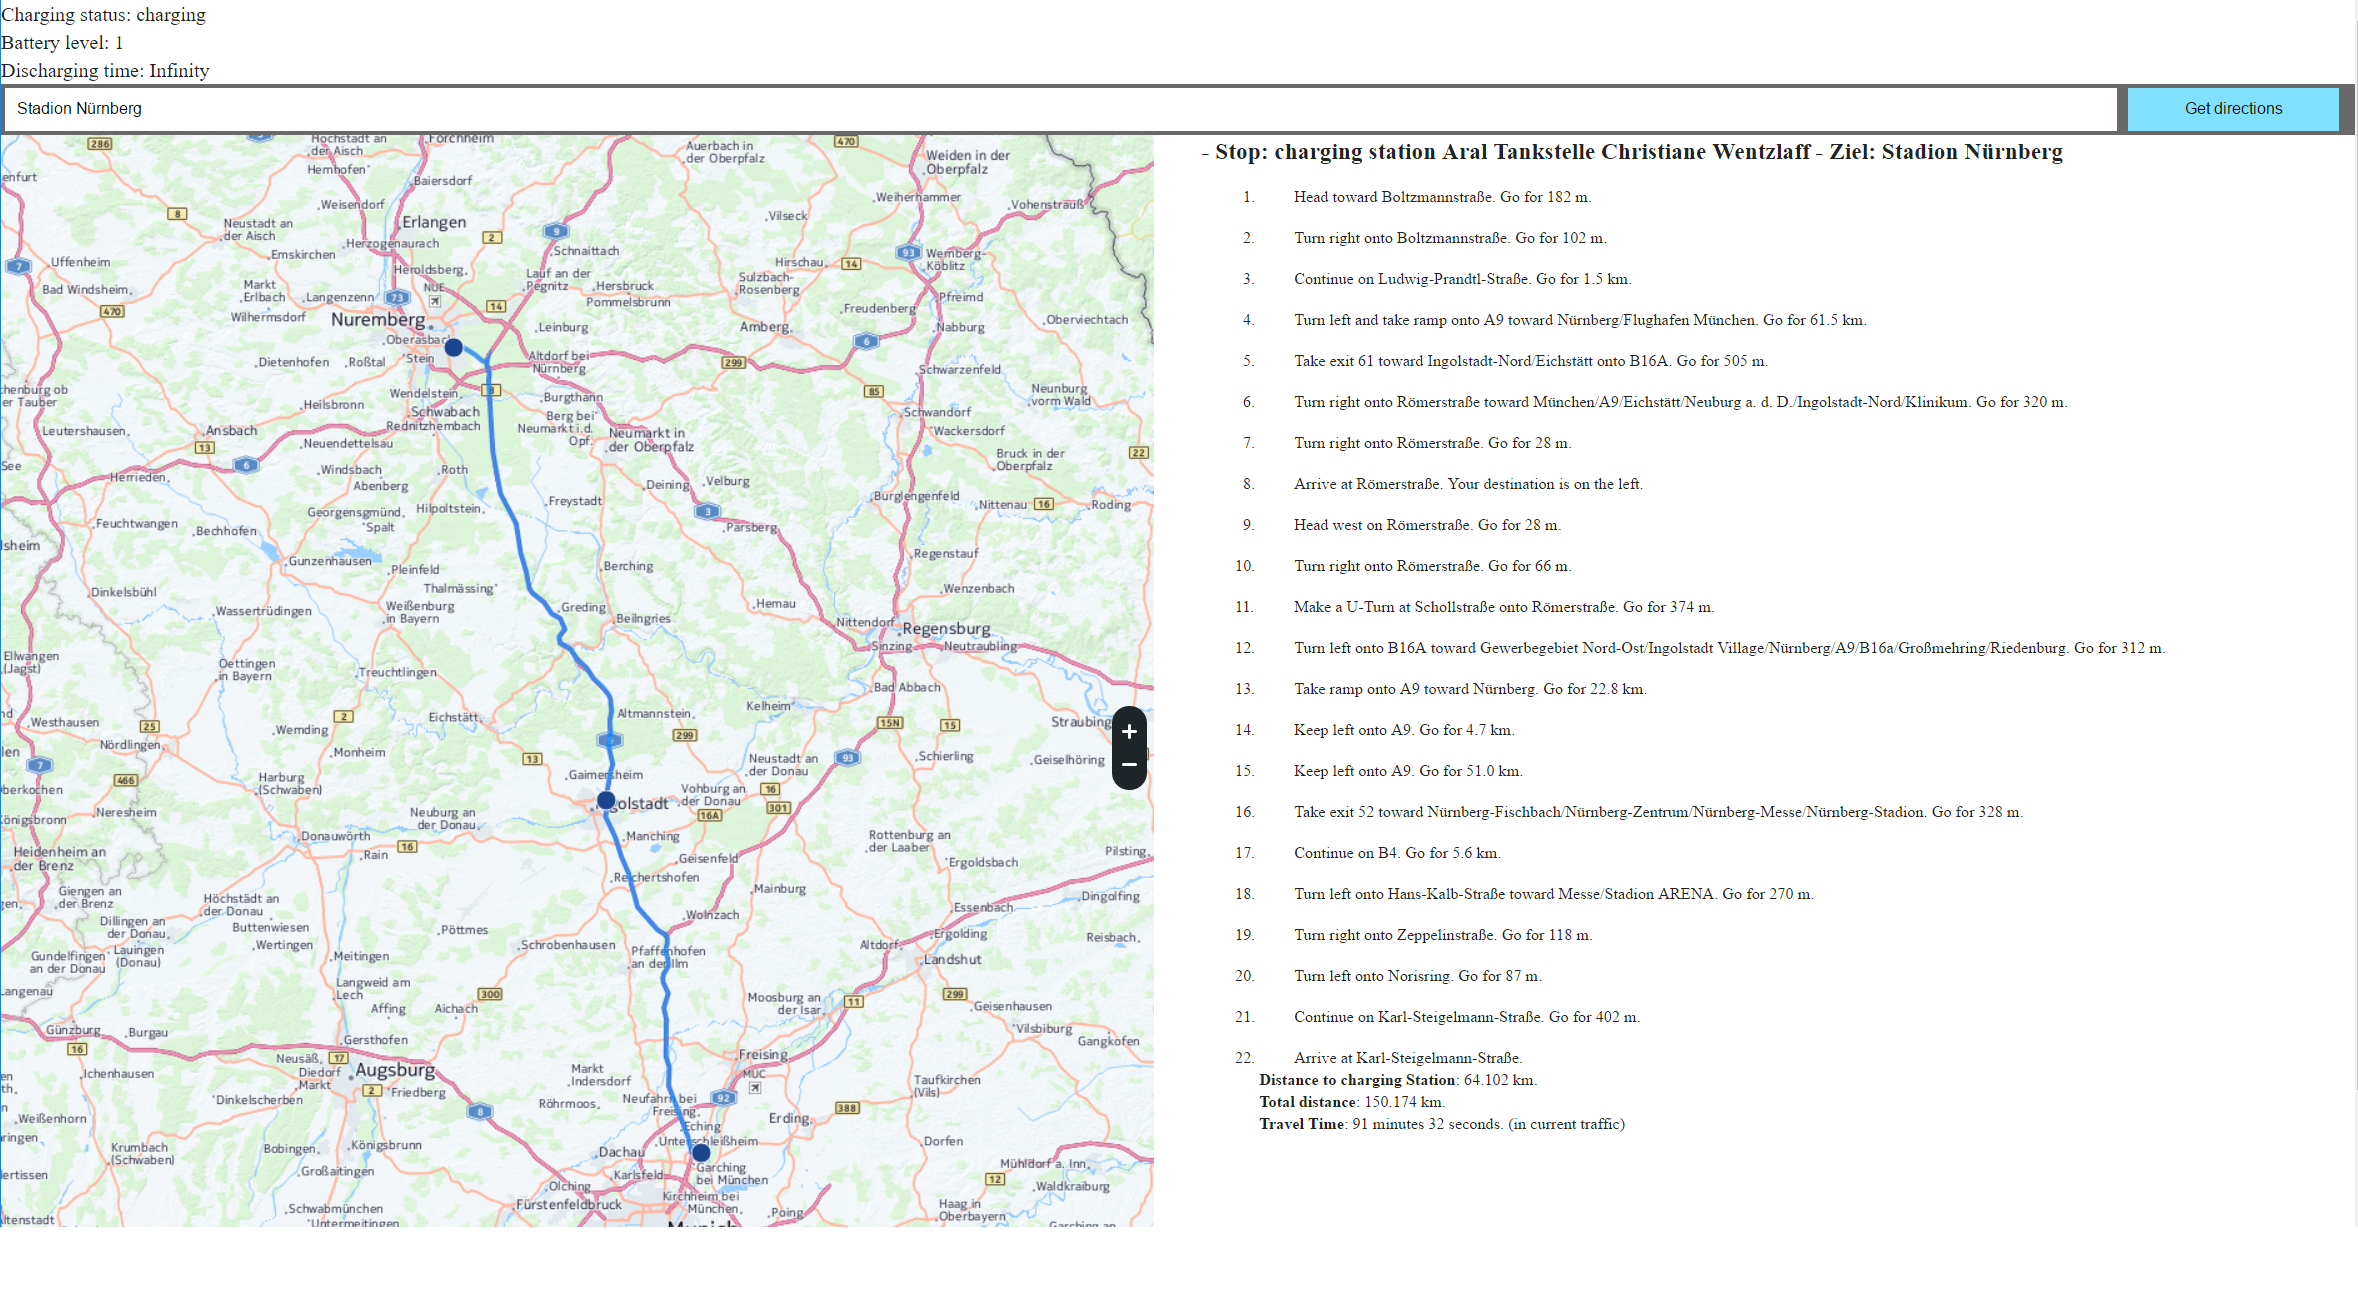
\includegraphics[width=0.46\textwidth]{user_interface}
\caption{User Interface}
\end{figure}

On the left side is the map and the calculated route displayed, in this case from TU Munich to a stadium in Nuremberg, with one charging stop in the middle. At the top is further information about the battery status, for example the charging status and the battery level. On the right side is additional trip information, it is only displayed to show the commands which will then be spoken out by text to speech. These should not be displayed in a later version. On the bottom of the left side is further information about the trip like the total travel time and total distance. 


\subsection{Markup}

As it is the case for the Simulation Manager Interface, the .arkup needed to display the user interface is kept minimalistic. At the top are some div elements to display the battery status of the device. In this case, it is the battery level of the computer it is running on to show its charging status, the battery level and the time till it is fully discharged. If it cannot be read, it will display ``charging state unknown''.

\begin{minted}{html}
<!DOCTYPE html>

<html>
<head>
[...]
</head>

<body>
<div id="charging">(charging state unknown)</div>
<div id="level">(battery level unknown)</div>
<div id="dischargingTime">(discharging time unknown)</div>
<div id="chatbox"></div>
<button onclick="setButtonPressed();">Try it</button>
</div>

<div id="map" style="position:absolute; width:49%; height:100%; background:grey" ></div>
<div id="panel" style="position:absolute; width:49%; left:51%; height:100%; background:inherit" ></div>
[...]
\end{minted}

Below that are two div elements one to display the map and another one to display the panel. All the rest is in JavaScript.

\begin{minted}{html}
<head>
    <meta name="viewport" content="initial-scale=1.0, width=device-width" />

    <link rel="stylesheet" type="text/css" href=".../mapsjs-ui.css" />

    <script type="text/javascript" src=".../mapsjs-core.js"></script>
    <script type="text/javascript" src=".../mapsjs-service.js"></script>
    <script type="text/javascript" src=".../mapsjs-ui.js"></script>
    <script type="text/javascript" src=".../mapsjs-mapevents.js"></script>

    <style type="text/css">
        .directions li span.arrow {
            display:inline-block;
            min-width:28px;
            min-height:28px;
            background-position:0px;
            background-image: url("../img/arrows.png");
            position:relative;
            top:8px;
        }
        .directions li span.depart  {
            background-position:-28px;
        }
        .directions li span.rightUTurn  {
            background-position:-56px;
        }
        .directions li span.leftUTurn  {
            background-position:-84px;
        }
        .directions li span.rightFork  {
            background-position:-112px;
        }
        [...]
\end{minted}

For alignment css is used which is embedded in the head of the html file.

\subsection{Initialization}

\begin{minted}{javascript}
<script type="text/javascript" charset="UTF-8">
    window.onload = function () {
        function updateBatteryStatus(battery) {
            document.querySelector('#charging').textContent = battery.charging ? 'charging' : 'not charging';
            document.querySelector('#level').textContent = battery.level;
            document.querySelector('#dischargingTime').textContent = battery.dischargingTime / 60;
        }

        navigator.getBattery().then(function(battery) {
            // Update the battery status initially when
            // the promise resolves
            updateBatteryStatus(battery);

            // .. and for any subsequent updates.
            battery.onchargingchange = function () {
                updateBatteryStatus(battery);
            };

            battery.onlevelchange = function () {
                updateBatteryStatus(battery);
            };

            battery.ondischargingtimechange = function () {
                updateBatteryStatus(battery);
            };
        });
    };
\end{minted}

First, the battery panel is initiated and set, it will then automatically do subsequent updates. 


\subsection{Route calculation}

As soon as the backend has resolved the locations for optimal charging stops, they can be send as a list to Here Maps to get an optimal route from start \texttt{waypoint0} over potential charging stops \texttt{waypoint1} to destination \texttt{waypoint2}. The number of waypoints is not directly limited and can vary. Additional parameters such as avoiding certain areas, such as a city center, or setting the number of alternative routes can be configured. For a full documentation, have a look here \cite{driver-13}.

\begin{minted}{javascript}
function calculateRouteFromAtoB(platform) {
    var router = platform.getRoutingService(),
        routeRequestParams = {
            mode: 'fastest;car',
            representation: 'display',
            routeattributes: 'waypoints,summary,shape,legs',
            maneuverattributes: 'direction,action',

            // TU Munich
            waypoint0: '48.2626,11.6679',

            // Aral Petriol Station
            waypoint1: '48.7752,11.4595',

            // Stadion Nuremberg
            waypoint2: '49.4268,11.1255'
        };

    router.calculateRoute(
        routeRequestParams,
        onSuccess,
        onError
    );
}
\end{minted}

When the routing API was successful and gives a response, this function will be called. It then calls the different functions and hands over the route element to add the calculated route to the map, highlighting the waypoints and adding direction commands to a list. 

\begin{minted}{javascript}
function onSuccess(result) {

    var route = result.response.route[0];

    /*
     * The styling of the route response on the map is
     * entirely under the developer's control.
     *
     * A representative styling can be found the full
     * JS + HTML code of this example in the functions
     * below:
     */

    addRouteShapeToMap(route);
    addManueversToMap(route);

    addWaypointsToPanel(route.waypoint);
    addManueversToPanel(route);
    addSummaryToPanel(route);

    // ...
}

\end{minted}


\subsection{Route response}

\begin{figure}[htp]
\centering
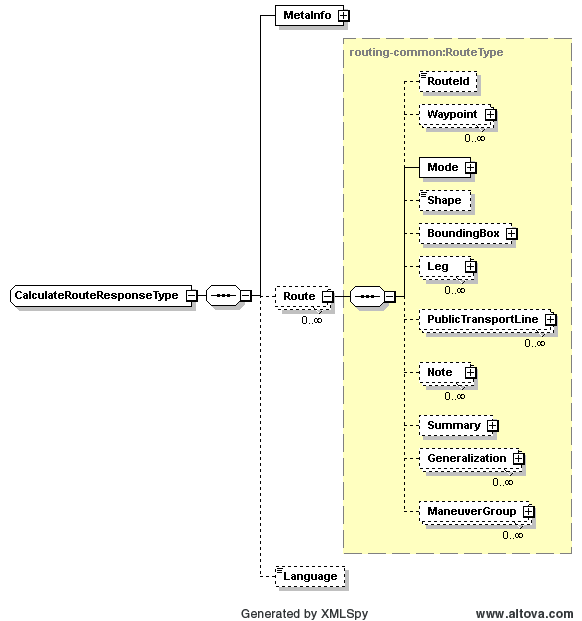
\includegraphics[width=0.46\textwidth]{route_response}
\caption{CalculateRouteResponseType \cite{driver-14}}
\end{figure}

As displayed in figure 1, the route response contains, besides meta info and information about language, the information set for the route. The route itself is stored in a route element, which can appear more than once depending on how many routes were calculated. 


\subsection{Summary Panel}

Here, further trip information is added to the panel which could also be extended to e.g. trip costs or energy used.

\begin{minted}{javascript}
function addSummaryToPanel(route){
    var summary = route.summary
    var summaryDiv = document.createElement('div'),
        content = '';
    var sum = [];

    sum[0] = 0;

    for (var i = 0;  i < route.leg.length; i += 1) {
        for (var j = 0;  j < route.leg[i].maneuver.length; j += 1) {
            sum[i]= sum[i] + route.leg[i].maneuver[j].length
        }
    }

    content += '<b>Distance to charging Station</b>: '+ sum[0]/1000 + ' km. <br/>';
    content += '<b>Total distance</b>: ' + summary.distance/1000  + ' km. <br/>';
    content += '<b>Travel Time</b>: ' + summary.travelTime.toMMSS() + ' (in current traffic)';

    summaryDiv.style.fontSize = 'small';
    summaryDiv.style.marginLeft ='5%';
    summaryDiv.style.marginRight ='5%';
    summaryDiv.innerHTML = content;

    routeInstructionsContainer.appendChild(summaryDiv);
}
\end{minted}

Further information about the trip is added to the panel here. For example, direction commands which could be used for text to speech. In the prototype, they are displayed to show the commands but later on they should not be displayed since it is distracting.

\begin{minted}{javascript}
function addManueversToPanel(route) {

    var nodeOL = document.createElement('ol'), i, j;

    nodeOL.style.fontSize = 'small';
    nodeOL.style.marginLeft ='5%';
    nodeOL.style.marginRight ='5%';
    nodeOL.className = 'directions';

    // Add a marker for each maneuver
    for (i = 0;  i < route.leg.length; i += 1) {
        for (j = 0;  j < route.leg[i].maneuver.length; j += 1) {

            // Get the next maneuver.
            maneuver = route.leg[i].maneuver[j];

            var li = document.createElement('li'),
              spanArrow = document.createElement('span'),
              spanInstruction = document.createElement('span');

            spanArrow.className = 'arrow '  + maneuver.action;
            spanInstruction.innerHTML = maneuver.instruction;
            li.appendChild(spanArrow);
            li.appendChild(spanInstruction);

            nodeOL.appendChild(li);
        }
    }

    routeInstructionsContainer.appendChild(nodeOL);
}
\end{minted}

\begin{minted}{javascript}
Number.prototype.toMMSS = function () {
    return Math.floor(this / 60) + ' minutes ' + (this % 60)  + ' seconds.';
}
\end{minted}

This function can open and display an information bubble at a geo position, for example information about the queue times at a charging stop provided by the backend. Furthermore, a notification can be raised for example if the energy consumption is too high or the battery is running low. 


\subsection{Notification Message}

\begin{minted}{javascript}
function openBubble(position, text){
    if(!bubble){
        bubble = new H.ui.InfoBubble(
            position,
            // The FO property holds the province name.
            {content: text});
        ui.addBubble(bubble);
    } else {
        bubble.setPosition(position);
        bubble.setContent(text);
        bubble.open();
    }
}
\end{minted}

\subsection{Adding the Route and the Waypoints to the Map}

Here, a series of \texttt{H.map.Marker} points from the route is created and added to the map. Furthermore, all the manuevers are then added to be displayed on the map.

\begin{minted}{javascript}
function addRouteShapeToMap(route){

    var strip = new H.geo.Strip(),
        routeShape = route.shape,
        polyline;

    routeShape.forEach(function(point) {
        var parts = point.split(',');
        strip.pushLatLngAlt(parts[0], parts[1]);
    });

    polyline = new H.map.Polyline(strip, {
        style: {
            lineWidth: 4,
            strokeColor: 'rgba(0, 128, 255, 0.7)'
        }
    });

    // Add the polyline to the map
    map.addObject(polyline);

    // And zoom to its bounding rectangle
    map.setViewBounds(polyline.getBounds(), true);
}
\end{minted}


\begin{minted}{javascript}
function addManueversToMap(route){
    var svgMarkup = '<svg width="18" height="18" ' +
            'xmlns="http://www.w3.org/2000/svg">' +
            '<circle cx="8" cy="8" r="8" ' +
            'fill="#1b468d" stroke="white" stroke-width="1"/>' +
            '</svg>',
        dotIcon = new H.map.Icon(svgMarkup, {anchor: {x:8, y:8}}),
        group = new  H.map.Group(),
        i,
        j;

    var marker1 =  new H.map.Marker({
            lat: 48.2626,
            lng: 11.6679} ,
        {icon: dotIcon});
    group.addObject(marker1);

    var marker2 =  new H.map.Marker({
            lat: 48.7752,
            lng: 11.459} ,
        {icon: dotIcon});
    group.addObject(marker2);

    var marker3 =  new H.map.Marker({
            lat: 49.4268,
            lng: 11.1255} ,
        {icon: dotIcon});
    group.addObject(marker3);

    group.addEventListener('tap', function (evt) {
        map.setCenter(evt.target.getPosition());
        openBubble(
            evt.target.getPosition(),
            evt.target.instruction);
    }, false);

    // Add the maneuvers group to the map
    map.addObject(group);
}
\end{minted}


\bibliographystyle{template/ACM-Reference-Format}
\bibliography{template/sigproc}

\end{document}
